\documentclass[12pt]{article}
\usepackage{algos-tasks}

\usepackage{colortbl}

\definecolor{CM}{HTML}{F7D560}
\definecolor{PP}{HTML}{DDA0DD}
\definecolor{MS}{HTML}{FF684F}
\definecolor{MP}{HTML}{00C6FC}
\definecolor{RG}{HTML}{78C279} 
\definecolor{MW}{HTML}{F3FFFF} 

\begin{document}
\task[regular]{Chess Tournament}
\begin{question}
UNSW is hosting a chess tournament for $n$ players, where every player will play every other player exactly once. You have been tasked with analysing the abilities of the players to predict who will win. Each player has been given two attributes: their talent $t_i$, and their workrate $w_i$.
You can assume that all the values of $t_i$ and $w_i$ are distinct. As an example, suppose we have the following six players, illustrated using both a table and scatter plot.

\begin{center}
\renewcommand{\arraystretch}{1.3}
\begin{tabular}{m{8cm}m{8cm}}
\raisebox{3cm}{\begin{tabular}{|c|c|c|}
    \hline
    Name & Talent ($t_i$) & Workrate ($w_i$)\\
    \hline
    \cellcolor{MS} Alice & 6 & 8\\
    \hline
    \cellcolor{MP} Bob & 2 & 1\\
    \hline
    \cellcolor{CM} Carlos & 8 & 5\\
    \hline
    \cellcolor{RG} David & 1 & 7\\
    \hline
    \cellcolor{PP} Erin & 5 & 2\\
    \hline
    \cellcolor{MW} Frank & 7 & 6\\
    \hline
    
\end{tabular}}
&{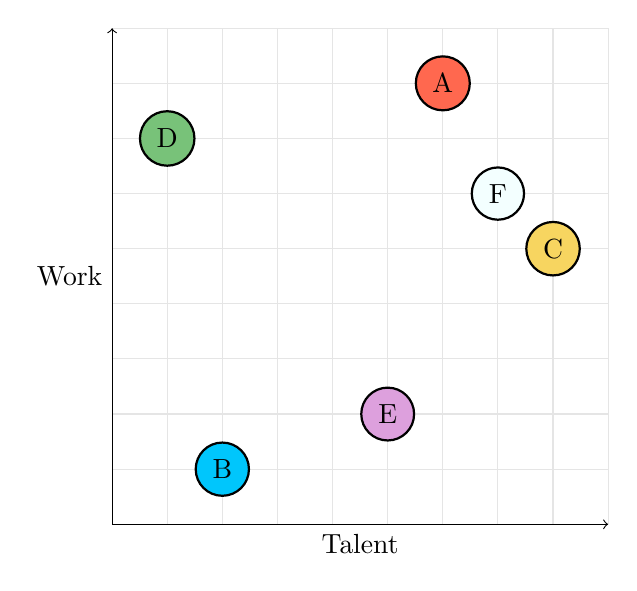
\begin{tikzpicture}[every node/.style={draw, circle, minimum size=0.2}, scale=0.7]
    \draw[gray!20] (0,0) grid (9,9);
    \node[thick,fill=MS] (A) at (6, 8) {A};
    \node[thick,fill=MP] (B) at (2, 1) {B};
    \node[thick,fill=CM] (C) at (8, 5) {C};
    \node[thick,fill=RG] (D) at (1, 7) {D};
    \node[thick,fill=PP] (E) at (5, 2) {E};
    \node[thick,fill=MW] (F) at (7, 6) {F};
    \draw[->] (0, 0) -- node[below,rectangle,draw=none]{Talent} ++(9, 0);
    \draw[->] (0, 0) -- node[left,rectangle,draw=none]{Work} ++(0, 9);
\end{tikzpicture}}
\end{tabular}
\end{center}

\begin{enumerate}[label = (\alph*)]
    \item \label{part a} We know that in a game between player $i$ and player $j$, if player $i$ is both less talented than player $j$, and not working as hard as player $j$, then player $j$ will definitely win the game. Otherwise, we do not know what the outcome of the game will be. 
    
    If a player is not guaranteed to lose any games, we call them a \emph{dominant} player. Design and analyse an $O(n\log n)$ algorithm that finds all of the dominant players in the tournament.

    \textbf{Hint:} There is both a divide-and-conquer solution and an arguably simpler alternative.

    \textbf{Hint:} In the example above, there are 3 dominant players: Alice, Carlos, and Frank.

    \item \label{part b} The less we know about the outcome of the tournament, the more exciting it will be to watch. We would like to know how many of the matches do not have a definite winner. Design and analyse an $O(n\log n)$ algorithm that counts the number of unpredictable matches.

    \textbf{Hint:} This is the number of pairs of players $(i,j)$ where $t_i < t_j$ and $w_i > w_j$.
    
    \textbf{Hint:} In the example above, 7 matches do not have a definite winner: {(A,C), (A,F), (B,D), (C,D), (C,F), (D,E) and (D,F)}. Since each pair plays once, \((j,i)\) is the same as \((i, j)\).

\end{enumerate}
\end{question}

\begin{rubric}
    \begin{enumerate}
        \item \begin{itemize}
            \item Design an algorithm that finds all the required players, and runs in $O(n \log n)$ time
            \item Justify that the algorithm is correct. That is, show that your algorithm includes a person \textbf{if and only if} they are able to win all of their matches.
            \item Justify that your algorithm runs in $O(n \log n)$ time.
            \item Expected length: half a page.
        \end{itemize}
        \item \begin{itemize}
            \item Design an algorithm that counts the number unpredictable matches, and runs in $O(n \log n)$ time.
            \item Justify the correctness and time complexity of your algorithm.
            \item Expected length: half a page.
        \end{itemize}
    \end{enumerate}
\end{rubric}

\begin{solution}
\end{solution}

\begin{attribution}
\end{attribution}

\end{document}